\documentclass{article}
\usepackage[utf8]{inputenc}
\usepackage{graphicx}
\usepackage{hyperref}
\usepackage[margin=2cm]{geometry}
\usepackage{circledsteps}

\title{COMP3030J Software Engineering Project 2 - 2023-2024 \\ Group 9}


% \textbf{Lecturer \& Supervisor:}\\
% Dr. Catherine Mooney\\
% Dr. Brett Becker

% \textbf{TA:}\\
% Shi Huilin

\author{Group 9\\
Peiang Miao (21207476)\\
Yitong Jl (21207468)\\
Linglong Yu (21207457)\\
Tongyu wu (21207482)\\
Xing Yang (21207454)\\
Liangzi Wang (21207244)}
\date{}

\begin{document}

\maketitle
\pagenumbering{roman}
\tableofcontents
\newpage
\pagenumbering{arabic}

\section{Problem Statement}
New Century, renowned for its professional consulting services in environmental sustainability, faces the challenge of seamlessly integrating sustainability principles into its internal operations, particularly in the procurement of office supplies and equipment. As a leading environmental consulting firm, New Century is dedicated to assisting clients in reducing their carbon footprint and adopting sustainable business practices. However, ensuring that the company's own procurement practices align with its sustainability values presents a significant hurdle.

The primary objective for New Century is to establish an efficient procurement process that not only guarantees the selection of products and services meeting stringent environmental standards but also effectively manages and approves procurement requests while tracking the environmental impact of such activities in real-time. This entails the careful selection of environmentally friendly office supplies and high-performance equipment, ensuring that each purchase aligns with the company's commitment to environmental protection.

The challenge lies in developing a transparent, efficient, and sustainable procurement system that reflects New Century's dedication to sustainability throughout its business operations. Achieving this goal is essential for New Century to uphold its sustainability commitments and maintain its reputation as a leader in environmental consulting services.

\begin{figure}[h]
    \centering
    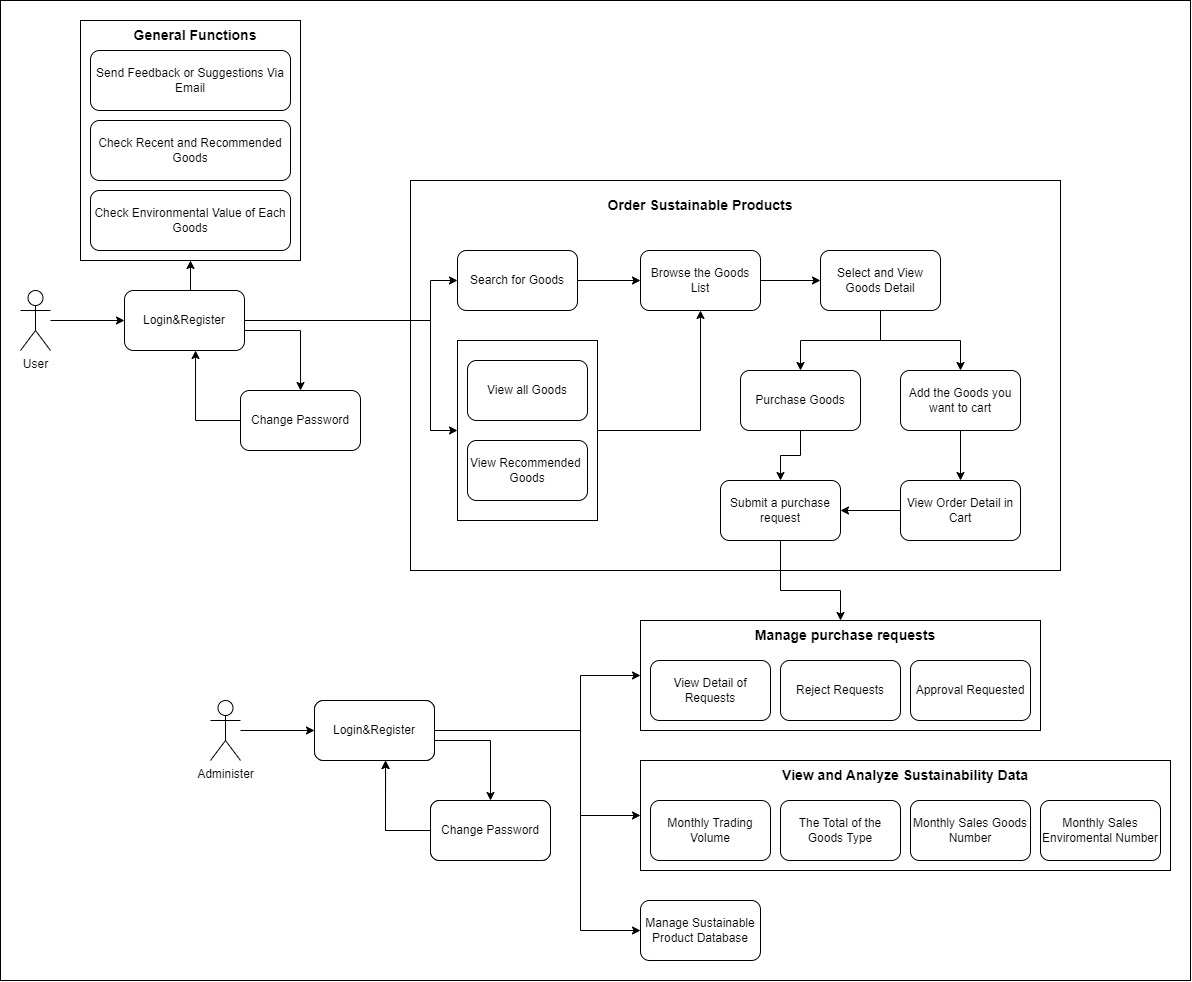
\includegraphics[width=1\textwidth]{figure1.png}
    \caption{All functions currently implemented}
    \label{image-myimage}
    \end{figure}

\section{Customer Portal}
\subsection{Home Page}
\subsubsection{Display product information}
According to the obtained product information, multiple product cards are displayed on the page. Among them, the first two items are displayed in the form of big cards, and the latter items are displayed in the form of ordinary cards. Each card contains a picture, name, and brief description of the item. In addition, there is a carousel display at the top of the page, showing the main product images. Switch every five seconds. Provides users with the ability to quickly browse products.

\subsubsection{Navigation bar}
Users can click on various options in the navigation bar to navigate to different pages.
\begin{enumerate}
    \item Goods page: Users can browse the details of products, including product information display, image display, purchasing and bookmarking functions, as well as related product recommendations.
    \item Faculty page: Shopping cart page (bookmarking product interface), allowing users to conveniently view and manage the products in the shopping cart.
    \item Value page:
    \item Support page: Provides users with an opportunity to contact the service team.
    \item Administer page: Mainly used for administrators to manage product information, view sales data, and process orders.
    \item Login page: Users can log in or register an account, as well as change passwords.
    \item Search function: Search based on the tags entered by the user, and display the search results in card form, providing functions for viewing more details and browsing through pagination.
    \item Logout: Click on the blue icon in the upper right corner of the webpage to log out.
\end{enumerate}

\subsubsection{Search bar}
\begin{enumerate}
    \item Obtain search information: Click on the input box in the upper right corner of the webpage, enter product keywords, and click the search button on the right to perform product queries, and display relevant product information based on the search results.
    \item Display search results: Based on the obtained product information, a series of product cards are displayed on the page. Each product card contains the product's image, name, and brief description, and provides a function to click to view more details.
\end{enumerate}

\subsection{Login and Register Page}
\begin{enumerate}
    \item Click the "Login" button in the navigation bar to enter the login interface.
    \item User login: Users can enter their username and password to log in. Both the username and password are required, and if left blank, corresponding error messages will be displayed.
    \begin{itemize}
        \item Password visibility: When entering the password, users can click the eye icon to toggle the visibility of the password.
        \item Click the "Login" button to log in. If the login is successful, the user will be automatically redirected to the homepage (HomePage); otherwise, a notification message indicating username or password validation error will be displayed.
    \end{itemize}
    \item Click the "Change your password." link to navigate to the password change page (ChangePage).
    \begin{itemize}
        \item Change password: Users can fill in their username, current password, new password, and confirm the new password to change their password. All fields are required, and the passwords entered twice must match, otherwise corresponding error messages will be displayed.
        \item Password visibility: When entering the new password, users can click the eye icon to toggle the visibility of the password.
        \item Click the "Change password" button to proceed with the change. If the change is successful, the user will be redirected to the login page (Login); if the change fails, a notification message indicating the account does not exist will be displayed.
    \end{itemize}
    \item Click the "Register for your ID." link to navigate to the registration page (Register).
    \begin{itemize}
        \item User registration: Users can fill in their real name, room number, email, phone number, password, and confirm password to register. All fields are required, and the passwords entered twice must match, otherwise corresponding error messages will be displayed.
        \item Password visibility: When entering the password, users can click the eye icon to toggle the visibility of the password.
        \item Information prompts: For the email input box, information prompts are provided to inform users that they will receive messages through this email.
        \item After clicking the "Register" button, if the registration is successful, the user will be redirected to the login page (Login); if the registration fails, a notification message indicating that the account already exists will be displayed.
    \end{itemize}
    \item Click the "Already have an administer ID? Click here" link to navigate to the administrator login page (AdminLogin).
    \begin{itemize}
        \item Administrators also have two interfaces for registration and login. The registration and login methods are the same as for users.
    \end{itemize}
\end{enumerate}

\subsection{Goods Page}
\begin{enumerate}
    \item Click the "Goods" button in the navigation bar, or hover over the product image on the homepage and click the "Detail" link to enter the Goods page.
    \item Display Product Information: Upon entering the Goods page, it displays basic information about the product, including product image, name, price, tags, environmental value, and description.
    \item Display Product Images: Hovering the mouse pointer over the image will display a preview tooltip. Clicking on the image at this time will enlarge the product image. By clicking on the buttons in the functional bar below the image, functionalities such as rotation and zooming of the image can be achieved. Clicking on a blank area will cancel the enlargement.
    \item Favorites: Users can click the favorite button to add or remove products from the shopping cart. Depending on the favorite status, the button icon will switch between favorite or unfavorite status. A red heart indicates the favorite status, while a gray heart indicates the unfavorite status.
    \item Purchase: Clicking the buy button allows users to submit a purchase request to the administrator.
    \item Product Recommendations: At the bottom of the page, it displays other products that users may be interested in based on the current browsing. Users can click to enter the details page of the selected product.
\end{enumerate}

\subsection{Faculty Page}
\begin{enumerate}
    \item Click the "Faculty" button in the navigation bar to enter the Faculty page. The Faculty page lists all the products that the user has favorited.
    \item Product Display: Each product in the shopping cart is displayed in the form of a card, including the product's image, name, brief description, price, and environmental value.
    \item Total Value Calculation: Based on the price of each product in the shopping cart, the total value of all products in the shopping cart is calculated and displayed in the upper right corner of the page.
    \item Purchase: Users can click the purchase button, but the specific purchase logic is not implemented in the code.
    \item Pagination: If there are too many products in the shopping cart, you can browse different pages of products through pagination. Click on specific page numbers or left and right arrows to switch pagination pages.
\end{enumerate}

\subsection{Value Page}

\subsection{Support Page}
\begin{enumerate}
    \item Click the "Support" button in the navigation bar to enter the Support page. The Support page provides users with the functionality to send emails to service providers to seek help and support.
    \item Email Sending Form: A form for sending emails is displayed on the page, where users can fill in their name, email, and message content, and then click the send button to send the email.
    \item Form Validation: The form performs required validation on the name, email, and message content fields. If the user does not fill in all fields, they will receive corresponding prompt messages.
    \item Sending Email: After clicking the send button, the page simulates the process of sending the email. The send button will display a loading state, and once the sending is completed, the button will return to its normal state.
    \item Success Message: After successful sending, the page will display the content of the sent email and clear the form, allowing users to continue filling in new emails.
    \item Bottom Navigation: The bottom of the page contains a fixed bottom navigation, allowing users to navigate back to other pages.
\end{enumerate}

\section{Administer Portal}
\subsection{Login Page}
\subsection{Administer Page}
\begin{enumerate}
    \item Click the "Administer" button in the navigation bar to enter the Administer page.
    \item Data Monitoring and Management: The page provides visual monitoring and management of system data, helping administrators better understand and manage data in the system, analyze website usage, product purchase, environmental value changes, etc.
    \begin{itemize}
        \item Monthly Transaction Volume Statistics: The page displays a line chart to show the transaction volume of the system each month. Users can understand the change trend of the system transaction volume through this chart.
        \item Product Type Distribution: The page displays a pie chart to show the distribution of different types of products in the system. Users can understand the proportion of various types of products in the system through this chart.
        \item Monthly Sales Quantity Statistics: The page displays a bar chart to show the sales quantity of the system each month. Users can understand the change in the quantity of products sold by the system through this chart.
        \item Monthly Sales Environmental Value Statistics: The page displays another line chart to show the sales environmental value of the system each month. Users can understand the change trend of the system sales environmental value through this chart.
        \item Data Table Display: The page displays a data table listing the product information in the system, including product name, price, address, tags, etc. Users can view and manage product data in the system through this table.
    \end{itemize}
    \item Handling User Purchase Requests: Located below the data analysis module, a table containing name, value, address, and tags is displayed, along with action buttons such as view details, delete, and confirm.
    \begin{itemize}
        \item Clicking the "Detail" button pops up a window to view detailed information about the order.
        \item Clicking the "Delete" button rejects the order.
        \item Clicking the "Confirm" button approves the order, officially purchasing the ordered products.
    \end{itemize}
    \item Add Product Information:Add Product Information: Administrators can click on the plus icon at the bottom right corner of the webpage to open a drawer on the right side. The drawer contains a form where users can input details such as the name, brief description, tags, value, and full description of the product, as well as upload a product image.

\end{enumerate}

\end{document}
